% Preference pair as geometry.
% Two activations h_chosen (near the reward axis) and h_rejected (further off it).
% The reward margin is the projection of (h_chosen - h_rejected) onto w_r:
% it is just the gap between where the two land on the reward axis.
% Compile with ../build_figures.sh -> content/assets/figures/preference-geometry.svg
\documentclass[border=10pt]{standalone}
\usepackage{tikz}
\usetikzlibrary{calc,arrows.meta}
\definecolor{rlink}{HTML}{3F51B5}    % reward direction
\definecolor{raccent}{HTML}{FF5722}  % the margin
\definecolor{rmuted}{HTML}{6B7280}
\begin{document}
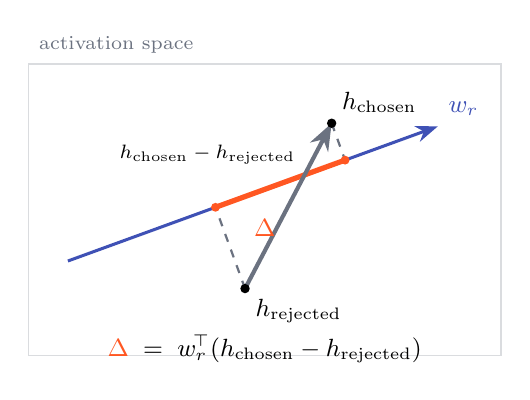
\begin{tikzpicture}[>=Stealth, line width=0.9pt, font=\small]
  \coordinate (O)  at (0,0);
  \coordinate (W)  at (20:5.0);
  \coordinate (HC) at (3.35,1.75);    % h_chosen
  \coordinate (HR) at (2.25,-0.35);   % h_rejected
  \coordinate (FC) at ($ (O)!(HC)!(W) $);   % foot of h_chosen on the reward axis
  \coordinate (FR) at ($ (O)!(HR)!(W) $);   % foot of h_rejected on the reward axis

  % activation-space frame
  \draw[rmuted!25, line width=0.6pt] (-0.5,-1.2) rectangle (5.5,2.5);
  \node[rmuted, font=\scriptsize, anchor=south west] at (-0.5,2.5) {activation space};

  % reward direction (thin, so the orange margin reads on the axis)
  \draw[rlink, ->, line width=1.1pt] (O) -- (W) node[above right, rlink] {$w_r$};

  % orthogonal drops from each activation onto the reward axis
  \draw[rmuted, dashed, line width=0.8pt] (HC) -- (FC);
  \draw[rmuted, dashed, line width=0.8pt] (HR) -- (FR);

  % the margin: the projection of the difference, i.e. the gap between the feet
  \draw[raccent, line width=1.9pt] (FR) -- (FC);

  % difference vector h_chosen - h_rejected
  \draw[rmuted, ->, line width=1.5pt] (HR) -- (HC);
  \node[anchor=east, black, font=\scriptsize] at (3.02,1.35)
     {$h_{\mathrm{chosen}}-h_{\mathrm{rejected}}$};

  % the two activations
  \fill (HC) circle (1.7pt) node[above right, black] {$h_{\mathrm{chosen}}$};
  \fill (HR) circle (1.7pt) node[below right, black] {$h_{\mathrm{rejected}}$};
  \fill[raccent] (FC) circle (1.6pt);
  \fill[raccent] (FR) circle (1.6pt);

  % margin label (below the orange segment, clear of the difference vector)
  \node[raccent, anchor=north] at (2.5,0.66) {$\Delta$};

  % the takeaway
  \node[anchor=north, font=\small] at (2.5,-0.8)
     {$\textcolor{raccent}{\Delta}\;=\;w_r^{\!\top}\!\left(h_{\mathrm{chosen}}-h_{\mathrm{rejected}}\right)$};
\end{tikzpicture}
\end{document}
